\documentclass[12pt]{article}
\usepackage{amsmath}
\usepackage[utf8]{inputenc}
\usepackage{breqn}
\usepackage{graphicx}
\usepackage[export]{adjustbox}
\newcommand*{\1}{\hspace{1pt}}
\graphicspath{/home/susmita/Documents/project/amar project}

\begin{document}

    \subsection*{Introduction}
    Theoreticians have briefed the significance of the mixing properties of binary liquid alloys 
    from both the scientific and the technological points of view. A precise understanding of 
    the mixing properties and phase diagrams of the alloy system is elementary to establish a 
    good arrangement between the experimental results, theoretical approaches, and empirical 
    models for liquid alloys with a miscibility gap.
    All liquid binary alloys can be grouped into two distinct classes that either exhibit 
    positive deviation(usually called segregating systems) or negative deviation (i.e. 
    short-ranged ordered alloys) from Raoult's law or the additive rule of mixing. If the 
    deviations are considerably large, they may conduct either phase separation or compound 
    formation in the binary system. \\

        There are liquid alloys, however, which do not belong exclusively to any of the above 
    two classes. For instance, the excess Gibbs energy of mixing $(G ^{xs} _{M} )$ for Cd–Na, and 
    Ag–Ge is negative at certain compositions, while positive at other compositions. In 
    liquid alloys such as Au–Bi, Bi–Cd, and Bi–Sb, the enthalpy of mixing $H_{M}$ is a 
    positive quantity but $G^{xs} _{M}$  is negative. Bi–Pb has positive $H_{M}$ and $G^{xs}_{M} $ in the 
    solid phase as against the negative values of $H_{M}$ and $G^{xs} _{M}$ in the liquid phase. 
    Systems such as Au–Ni and Cr–Mo exhibit immiscibility in the solid phase which is not 
    visible in the interrelated liquid phase. Systems such as Ag–Te show intermetallic 
    phases and large negative $H_{M}$ values in the liquid phase concurrently with a liquid 
    miscibility gap. \\

    
        Systems such as Al–Bi, Al–In, Al–Pb, Bi–Ga, Bi–Zn, Cd–Ga, Ga–Pb, Ga–Hg, Pb–Zn, Pb–Si 
    and Cu–Pb, etc, are represented by liquid miscibility gaps and exhibit enormous positive 
    $H_{M}$. Their properties in the liquid phase tend to vary markedly as a role of composition (c),
    temperature (T ), and pressure (p). The long-wavelength limit (q→0)of the 
    composition–composition structure factors, $S_{cc}$ (0) diverges as the composition and 
    temperature approach the critical values c → $c_{c}$, and T → $T_{c}$. $S_{cc}$ (0), which can instantly
    be obtained from thermodynamic functions (either acquired by taking the first composition 
    derivative of the activity or through the second derivative of the Gibbs function), is 
    very useful for establishing the immiscibility and the degree of segregation in binary 
    liquid alloys. Additional thermodynamic, structural, and transport properties are also 
    found to alter anomalously in the area of $c_{c}$ and $T_{c}$. \\ 


        A provided unary system is expressed by two pairs of independent variables, namely 
    the mechanical degrees of freedom (pressure (p) or volume ($\Omega$)) and the thermal 
    degrees of freedom (temperature (T) or entropy (S)). The preference of independent 
    variables is mostly a concern of free option; yet, there are four possibilities for 
    creating such pairs have one mechanical and one thermal variable, say (S,$\Omega$ ), 
    (S, p), (T, $\Omega$) and (T, p). These pairs guide to thermodynamic functions such as 
    internal energy E(S,$\Omega$), enthalpy H (S, p), Helmholtz energy F (T, $\Omega$), and 
    Gibbs energy G(T, p), respectively.\\

    The enthalpy, H, merging the internal energy E to the mechanical degrees of freedom
    (p, $\Omega$) is\\
                    
                 \begin{equation}
                    H = E + p\Omega
                \end{equation}

    or in differential form,
                
                \begin{equation}
                    dH = \delta Q + \Omega dp
                \end{equation}

    where       \begin{equation*}
                    \delta Q = dE + pd \Omega
                \end{equation*}

    The Helmholtz energy, F, relates E to the thermal degrees of freedom (S,T), i.e.\\

                \begin{equation}
                    F = E - TS
                \end{equation}

    or,

                \begin{equation}
                    dF = -SdT - pd \Omega
                \end{equation}

    In the case of reversible isothermal and isochoric processes (T , $\Omega$ = constant),
    dF = 0, i.e.
    F remains invariant.
        Similarly, the Gibbs function establishes a relation between H and the thermal degrees
    of freedom, i.e.\\

                \begin{equation}
                G = H - TS
                \end{equation}

or

                \begin{equation}
                dG = -S dT + \Omega dp
                \end{equation}

    In the case of a reversible isothermal reaction at constant pressure (T , p = constant),
    dG = 0, i.e. G remains invariant.\\

        Also, H , F and G can readily be used to obtain the heat capacity C ($C_{p}$ or $C_{\Omega}$ ),
    entropy, isothermal ($\chi _{T}$ ) and adiabatic ($\chi _{S}$) compressibilities, the volume and the volume
    expansivity ($\alpha  _{p}$):\\

    \begin{align}
    &  C_{p} = \left(\frac{\partial H }{ \partial T}\right)_{p} = T \left(\frac{\partial S}{\partial T} \right) _{p} = -T \left(\frac{\partial ^2 G }{ \partial T^2}\right) _p \\
    & C_{\Omega} = \left(\frac{\partial E }{ \partial T}\right)_{\Omega} = T \left(\frac{\partial S}{\partial T} \right) _{\Omega} = -T \left(\frac{\partial ^2 F }{ \partial T^2}\right) _\Omega \\
    & S = \left(\frac{\partial G }{ \partial T}\right)_{p} =  \left(\frac{\partial F}{\partial T} \right) _{\Omega} \\
    & \Omega  = \left(\frac{\partial G }{ \partial p}\right)_{T} \\
    & \chi _T  \equiv  - \frac{1}{ \Omega} \left(\frac{\partial  \Omega }{ \partial p}\right)_{T} \\ 
    & \chi _S  \equiv  - \frac{1}{ \Omega} \left(\frac{\partial  \Omega }{ \partial p}\right)_{S} \\
    & \alpha  _p  \equiv  \frac{1}{ \Omega} \left(\frac{\partial  \Omega }{ \partial T}\right)_{p}  
    \end{align}\\

    At indicator, we furthermore have some important effects from isotherms of liquid–vapor phases which at the critical point must fulfill
    \begin{align}
    & \left(\frac{\partial p}{\partial \Omega} \right) _{T_{c}} = \left(\frac{\partial ^2 p}{\partial \Omega ^2} \right) _{T_{c}} =0
    \end{align}\\

    At T = $T_c$ , the following physical properties become infinite, i.e.\\


    \begin{align}
    & C_p = T \left(\frac{\partial S}{\partial T} \right) _p = \infty \\
    & \alpha _p = \frac{1}{\Omega} \left(\frac{\partial \Omega}{\partial T} \right) _p = \infty \\
    & \chi _T = -\left(\frac{\partial \Omega}{\partial p} \right) _T = \infty 
    \end{align}\\

    For a binary mixture, such as an A–B alloy consisting of $c_A$ moles of component A and $c_B$
    moles of component B, rather than guiding to the fundamental values of their function, 
    we define the function of mixing. For example, the Gibbs energy of mixing, $G_M$ , is represented as

    \begin{equation}
        G_M = G(alloy) - c_A G^{0}_{A} - c_B G^{0}_{B}
    \end{equation}

where $G ^{0}_{A}$ and $G ^{0}_{B}$ are the Gibbs free energy of the two pure components. Equivalent
definitions also exist for HM , SM and other functions.The integral quantities can also be divided 
into the partial quantities, i.e.

    \begin{equation}
        G_M = c_A \overline{G} _{M,A} + c_B \overline{G} _{M,B}
    \end{equation}
with
    \begin{equation}
        \overline{G} _{M,i} = RT ln a_i                \tag*{( i= A,B )}
    \end{equation}
where  $\overline{G} _{M,i} $ are the partial Gibbs energies and $a _{i}$ are the thermodynamic 
activities of the component i.
$G _M$ defines the stability of the phases in a binary mixture. The curves describing
$G _M$ against c deviation can, in general, have a shape like either curve a or curve b as displayed
in figure 1. For $G _M$ as in curve a, the homogeneous solution is stable at all values of c at
$T _1$ ; if not other phases (i.e. intermediate phases) in the system display more negative $G _M$
values.


    
\begin{adjustbox}{center,caption={A schematic diagram symbolizing the Gibbs energy of mixing at constant T plotted against concentration. 
    Curve a, complete mixing ($ T _1 < T _c $). 
    Curve b, incomplete mixing ($ T _2 < T _c $), 
    $\Delta c$ represents the miscibility gap at $ T _2$ .},label={somelabel},nofloat=figure,vspace=\bigskipamount}
    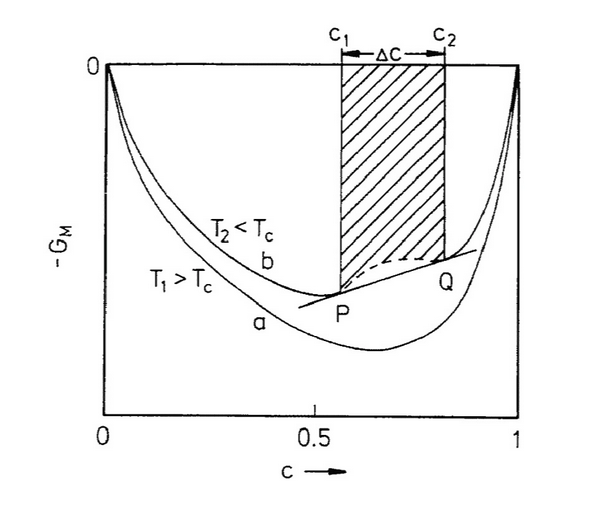
\includegraphics[width=0.7\textwidth]{fi_1}
\end{adjustbox}
    

    For curve b, the homogeneous solution is varying in the composition range $\Delta c$, because
$G _M$ can be reduced if the mixture separates into two phases. The composition of these phases
is provided by the points of contact P and Q of the common tangent line to the $G _M$(c) curve.
The reduced $G _M$  values of these two phases are given by this line. Within the composition
range $\Delta c$ only the portions of the two phases change if the total composition of the alloy
modifications. At P($c _1$) and Q($c _2$) the partial Gibbs energies of the components of both diverged
phases are equivalent,

    \begin{equation}
        \overline{G} _{M,i}(c _{1}) =  \overline{G} _{M,i}(c _{2})          \tag*{( i= A,B )}
    \end{equation}

    Hence P and Q indicate the limit of thermodynamic equilibrium. $G _M$ diverts as a function of
temperature from a concave to a convex surface for $\Delta c $ at the spinodal. The points of
inflection in the curves define the spinodal line. The critical composition and the critical
temperature are determined from the conditions at T = $T _c$\\

    \begin{align}
        \left(\frac{d^2 {G _M}}{d c^2} \right) _{c = c_c} = 0 \\
        \left(\frac{d^3 {G _M}}{d c^3} \right) _{c = c_c} = 0 
    \end{align}


    At this step, it should be pointed out that the long-wavelength limit (q → 0) of
the structure factor $S _{cc} $(q) which is well known as the
concentration fluctuation, $S _{cc} $(0), is also correlated to the thermodynamic function, i.e

    \begin{equation}
        S_{cc}(0) =  RT \left(\frac{d^2 G _M}{d c^2} \right) ^ {-1}_ {T,P}
    \end{equation}
As $ c\to c _c$ and $ T\to T_c $ ,one sees that

    \begin{equation}
        S_{cc}(0) \to \infty
    \end{equation}  
Thus, a phase separation in a binary mixture is signaled by a strong enhancement of the
concentration fluctuations. 
The ideal solution behavior (HM = 0) of a binary mixture is presented by
    \begin{equation}
        G ^ {id} _M = RT (c_A \ ln c_A + c_B \ ln c_B).
    \end{equation}

The distinctions in the thermodynamic behavior of a real binary solution and an ideal solution 
are represented by the excess quantities, i.e.
    \begin{equation}
        G ^ {xs} _M = G _M - G ^{id} _M
    \end{equation}

or using equation (5)

    \begin{equation}
        G ^ {xs} _M = H _M - T S ^{xs} _M
    \end{equation}
with
    \begin{equation}
        S ^{xs} _M = S _M + R (c _A \ ln c_A + c _B \ ln c _B)
    \end{equation}\\



\subsection*{Observable indicators}


Segregating liquid alloys\\

From the point of view of interatomic interactions, a binary alloy is either (i) an ordered
alloy, where unlike atoms are chosen as nearest neighbors over like atoms, or (ii) a
segregated alloy, where like atoms are chosen to pairs as nearest neighbors over unlike
atoms. Unfortunately, there is no direct way to distinguish the constituent atoms and
hence the identification of a nearest-neighbor pair of atoms is challenging. In this case
either the structural data or the experimental thermodynamic functions (such as activity, the heat of
mixing, excess Gibbs energy of mixing, excess heat capacity, etc) or other thermophysical
data (such as viscosity, diffusivity, density, surface tension, electrical resistivity, etc) are
supposed to extract information associated with interatomic interactions. Some of the
empirical criteria as well as microscopic parameters which are used to identify segregated
alloys are summarized below.\\
(a) Alloys displaying positive deviations from Raoult’s law.\\
(b) The heat of formation and the excess Gibbs energy of mixing are positive.\\
(c) The concentration fluctuation in the long-wavelength limit ($ S _{cc}(0) $) is greater than
    the ideal value.

    Table 1 provides a list of $G^{xs} _{M}$ , $H _M$ and $S^{xs} _{M}$ at the equiatomic composition 
of segregating liquid alloys which are arranged according to the type of their phase equilibria. Of these Bi–
Zn, Pb–Zn, Cu–Pb, Cd–Ga, Al–Bi, Al–In, Al–Pb, etc, exhibit liquid immiscibility. $G^{xs} _{M}$ and
$ H _M $ are comparatively large positive quantities. For these alloys only a few experimental
heat capacity data are available . The data, in general, show a decrease in Cp with increasing temperature. The energetic and structural effects in the
solution phase can be more directly seen by the excess heat capacity $\Delta  C _p $values:

    \begin{equation}
        \Delta  C _p = C_p(c) - c_A \ C_{p,A} - c_B \ C_{p,B} 
    \end{equation} 
    \\
    \\
    \\
    \\
    \\
    
$\Delta  C _p $ are positive and indicate maximum values near to $ T _c$ and $c _c$ . 
 
\begin{table}[t!]
\centering
\caption{Thermodynamic properties of liquid binary alloys at equiatomic composition displaying
segregation.}
 \begin{tabular}{|c c c c c c|} 
 \hline
 Alloys & Ref. & T (K) & $G ^ {xs} _ {M}$/RT & $H _M/RT$ & $S ^ {xs} _ {M}$/R \\ [0.5ex] 
 \hline\hline
 Al–Bi & (i) & 900 & 0.814 & 0.823 & 0.09 \\ 
 Al–In &     & 1150 & 0.54 & 0.49 & -0.05 \\
 Al–Pb &     & 1700 & 0.527 & 0.847 & 0.32 \\
 Bi–Ga & (ii) & 550 & 0.493 & 0.433 & -0.06 \\
 Bi–Zn &     & 880 & 0.36 & 0.60 & 0.24 \\ [1ex] 
 \hline
 \end{tabular}
\end{table}

\end{document}